% Define document class
%\documentclass[twocolumn]{aastex631}
\documentclass[modern]{aastex631}

% Some entries inspired from a preamble by Adrian Price-Whelan, https://github.com/adrn/PhaseSpiralAsteroseismology/blob/main/tex/preamble.tex

\usepackage{showyourwork}

% Latex imports
\let\tablenum\relax             % necessary for AASTeX
\usepackage{siunitx}
\sisetup{range-phrase=-, range-units=single, separate-uncertainty=true}
\sisetup{separate-uncertainty=true}
\usepackage{blindtext}          % Filler text
\usepackage{xcolor}

% paper comments
\usepackage{comment}						 % comments that can be switched visible/invisible
\includecomment{comment}
%\specialcomment{outtake}{\begingroup\sffamily\color{gray}}{\endgroup}
\specialcomment{note}{\begingroup\sffamily\color{red!40!green!70!blue!90}}{\endgroup}
%\excludecomment{note}                       % switch notes off

%% switch TODO notes on/off
\usepackage[backgroundcolor=red!20!green!40!blue!10, textsize=tiny]{todonotes}
\usepackage{regexpatch}
\makeatletter
\xpatchcmd{\@todo}{\setkeys{todonotes}{#1}}{\setkeys{todonotes}{inline,#1}}{}{}
\makeatother
%\usepackage[disable]{todonotes}			% switches all todo notes to invisible

% ---------------------------------
% PAPER VARIABLES
\newcommand{\Nplanets}{\ensuremath{733}}
\newcommand{\percentageTransiting}{999}
\newcommand{\dmax}{\ensuremath{50\,\mathrm{pc}}}
\newcommand{\wrr}{0.001}
\newcommand{\windowsize}{25}
\newcommand{\prSmin}{10}
\newcommand{\prSmax}{1000}
\newcommand{\prWRRmin}{10^{-5}}
\newcommand{\prWRRmax}{0.1}
\newcommand{\prRmin}{0.1}
\newcommand{\prRmax}{15}


% ---------------------------------
% CONSTANTS/MISSIONS/ABBREVIATIONS

% SIunitx definitions
\DeclareSIUnit\mSun{M_\odot}
\DeclareSIUnit\Msun{M_\odot}
\DeclareSIUnit\mStar{M_\star}
\DeclareSIUnit\Mstar{M_\star}
\DeclareSIUnit\mEarth{M_\oplus}
\DeclareSIUnit\Mearth{M_\oplus}
\DeclareSIUnit\rEarth{R_\oplus}
\DeclareSIUnit\Rearth{R_\oplus}
\DeclareSIUnit\year{yr}
\DeclareSIUnit\au{au}
\DeclareSIUnit\dex{dex}
\DeclareSIUnit\ppm{ppm}
\DeclareSIUnit\eV{eV}

% Missions/Projects/Packages
\newcommand{\project}[1]{\textsl{#1}}
\newcommand{\rst}{\project{Nancy Grace Roman Space Telescope}}
\newcommand{\plato}{\project{PLATO}}
\newcommand{\cheops}{\project{CHEOPS}}
\newcommand{\kepler}{\project{Kepler}}
\newcommand{\emcee}{\project{emcee}}

% Stats / probability
\newcommand{\given}{\,|\,}
\newcommand{\norm}{\mathcal{N}}
\newcommand{\pdf}{\textsl{pdf}}

% Maths
\newcommand{\dd}{\mathrm{d}}
\newcommand{\transpose}[1]{{#1}^{\mathsf{T}}}
\newcommand{\inverse}[1]{{#1}^{-1}}
\newcommand{\argmin}{\operatornamewithlimits{argmin}}
\newcommand{\mean}[1]{\left< #1 \right>}

% Non-scalar variables
\renewcommand{\vec}[1]{\ensuremath{\bs{#1}}}
\newcommand{\mat}[1]{\ensuremath{\mathbf{#1}}}

% Unit shortcuts
\newcommand{\msun}{\ensuremath{\mathrm{M}_\odot}}
\newcommand{\mjup}{\ensuremath{\mathrm{M}_{\mathrm{J}}}}
\newcommand{\kms}{\ensuremath{\mathrm{km}~\mathrm{s}^{-1}}}
\newcommand{\mps}{\ensuremath{\mathrm{m}~\mathrm{s}^{-1}}}
\newcommand{\pc}{\ensuremath{\mathrm{pc}}}
\newcommand{\kpc}{\ensuremath{\mathrm{kpc}}}
\newcommand{\kmskpc}{\ensuremath{\mathrm{km}~\mathrm{s}^{-1}~\mathrm{kpc}^{-1}}}
\newcommand{\dayd}{\ensuremath{\mathrm{d}}}
\newcommand{\yr}{\ensuremath{\mathrm{yr}}}
\newcommand{\AU}{\ensuremath{\mathrm{AU}}}
\newcommand{\Kel}{\ensuremath{\mathrm{K}}}

% Misc.
\newcommand{\bs}[1]{\boldsymbol{#1}}

% Astronomy
\newcommand{\feh}{\ensuremath{{[{\rm Fe}/{\rm H}]}}}
\newcommand{\mh}{\ensuremath{{[{\rm M}/{\rm H}]}}}
\newcommand{\logg}{\ensuremath{\log g}}
\newcommand{\Teff}{\ensuremath{T_{\textrm{eff}}}}
\newcommand{\vsini}{\ensuremath{v\,\sin i}}
\newcommand{\gaia}{\textsl{Gaia}}

% Begin!
\begin{document}

% Title
\title{The imprint of global magma oceans on exoplanet demographics}

% Author list
\author[0000-0001-8355-2107]{Martin Schlecker}
\affiliation{Department of Astronomy/Steward Observatory, The University of Arizona, 933 North Cherry Avenue, Tucson, AZ 85721, USA}
\author{al.}


% Abstract
\begin{abstract}
    $\ldots$ magma oceans $\ldots$

    Here, we assess the ability of space and ground-based telescopes to test this hypothesis using Bioverse, a simulation framework that leverages contextual information from the overall planet population.
    $\ldots$

%    We argue that in the near future, ESA's PLATO mission and NASA's Roman Space Telescope will be the most promising endeavors to constrain this demographic feature.
%    For each of these missions, we identify the key mission design drivers that enable a statistically sound detection.
%    We also show the unique synergy of these missions in answering this question, and what survey strategy optimizes the statistical power of the combined dataset.
%    $\ldots$ its measurement will also provide insights into which stars harbor the nearest habitable worlds.
\end{abstract}

% Main body
\section{Introduction}
\todo[inline]{papers: \citep[][statistical detection of GH transition]{Turbet2019}, \citep[][water loss, O2 buildup around M dwarfs]{Luger2015}, \citep[][Solubility of H in magma oceans]{Hirschmann2012,SchlichtingShahar_inreview,} \citet{Hamano2013,Hamano2015,Barth2021,Downey2022}.}



\begin{note}
(Several patterns in the planetary parameter space have been reported in demographic studies or predicted from planet formation theories.)
    Venus and Earth, while having accreted from the same mass reservoir and despite their similar bulk properties, evolved into planets with very different environmental conditions on their surfaces.
    At the formation of the Solar System, both planets underwent a giant impact phase [CITE!] that melted their mantles, leading to a magma ocean stage.
    Due to these similar early formation phases, it was commonly assumed that the divergence of Venus and Earth -- in particular Venus's water loss -- occurred late in their evolution~\citep{Elkins-Tanton2013}.
    \citet{Hamano2013} showed that such a late desiccation process is not needed to explain the stark differences: for a planet rich in volatiles and receiving high enough radiation levels from its host star, a steam atmosphere limits the outgoing radiation from the (molten) planetary surface.
    This runaway greenhouse state prevents the planet's rapid cooling and can extend the magma ocean stage to hundreds of \SI{}{\mega\year}, enough to remove the entire water reservoir from a rocky planet by hydrodynamic escape.
    \todo[inline]{important for motivating the existence of the pattern: ``the solidification timescale can become comparable to the main-sequence lifetime of the star (Hamano et al. 2013, 2015)'' \citep{Lichtenberg2022} }
    Under the right conditions, different orbital distances alone can thus decide about a planet's water content and ultimately its habitability.
    If received flux makes the difference between our own habitable planet and dry, dead Venus, there is good reason to believe that such patterns exist in exoplanet systems as well.

    ...long-term goal/overarching objective: derive the geophysical history of rocky extrasolar planets. More concrete: Constrain the limits of runaway greenhouse transitions, and thus the inner edges of the habitable zone. Also: How close is Earth from this runaway greenhouse irradiation limit?
   ...
\todo[inline]{introduce magma oceans and their influence on planetary radii~\citep{Dorn2021}.}
    ...current/future observations of planets that are currently in the runaway greenhouse phase may constrain properties of their planetary mantles... make connection between interior and atmospheres.
\end{note}



\section{Global magma oceans and their imprint on exoplanet demographics}
\todo[inline]{"Methods Section" for the geophysical models.\\
~\\
\textbf{Main assumptions:}\\
- Assume that every planet has \textit{some} water. Enough for runaway GH under the right conditions. Baseline water content: 20\% \\
- Limitation to small planets without significant atmospheric envelopes.\\
- we ignore water loss by H$_2$O photolysis in the upper atmosphere and subsequent H escape, which would eventually cool even planets within the runaway greenhouse regime~\citep{Lichtenberg2022}.\\
- we ignore tidal heating, which could extend the magma ocean phase of close-in planets (and change their orbits via tidal orbital evolution)( Jackson et al., 2008; Barnes et al., 2013 (?)).\\
}
\subsection{Global magma oceans}
\todo[inline]{introduce geophysical model.\\ Introduce its parametrization either here or further down when modeling demographic imprint.\\ Figure~\ref{fig:magmaocean_model} goes here.}

%\begin{figure}
\begin{figure}[!ht]
    \begin{centering}
        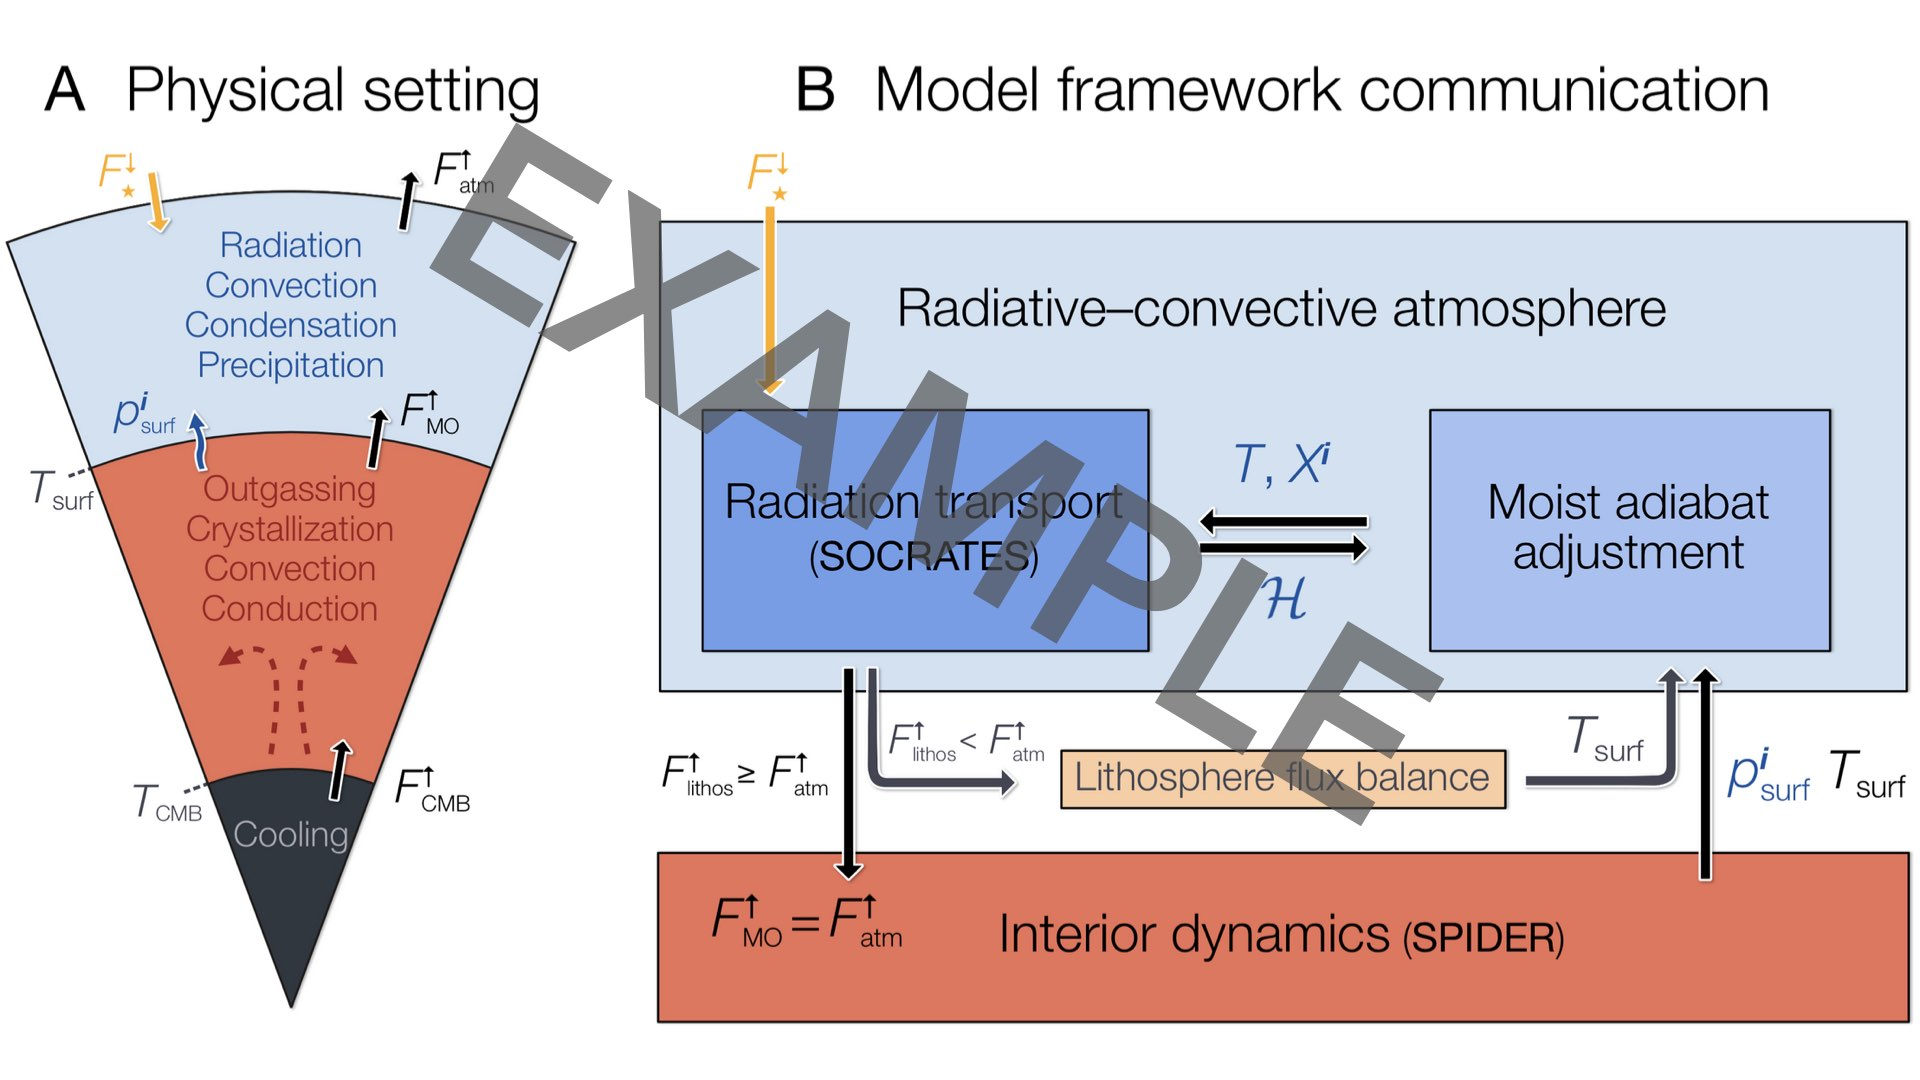
\includegraphics[width=\hsize]{figures/magmaocean_model.jpg}
        \caption{Schematics of the geophysical model framework.}
        \label{fig:magmaocean_model}
    \end{centering}
\end{figure}


\subsection{Demographic imprint of magma oceans}
\todo{describe the expected imprint on the exoplanet population. \\Provide parametrizations from \citet{Dorn2021}'s models.}

\subsubsection{Parametrization}
\label{sec:mo_model}
\todo{specific parametrization, dependency on bulk planet/orbit params (doesn't have to be its own subsubsection)}



\begin{note}
    The power from the host star per unit area at the position of a planet or instellation $S$ in units of Earth's insolation is given by
    \begin{equation}
        \frac{S}{S_\oplus} = \left(\frac{L_\star}{L_\odot}\right) \left(\frac{au}{a}\right)^2 .
    \end{equation}
    Here, we assume global redistribution of incoming flux and a fixed albedo of $0.3$, comparable to Earth's [CITE].
    The absolute value of $S_\oplus$, by which all synthetic planets are scaled, is then \SI{238}{\watt\per\square\meter}.
    We further define the solar-equivalent semi-major axis $a_{eff} = a (L_\star/L_\odot)^{-1/2}$, at which a planet experiences the same instellation as a Solar System planet at an orbital distance~$a$.
\end{note}





\section{Testing the magma ocean hypothesis}
\todo[inline]{Methods and results section of the hypothesis testing part. Introduce the idea of constraining magma ocean frequencies and/or physics with Bayesian stats on exoplanet population; introduce Bioverse; report methods of the hypothesis tests.\\
Caveats: see \citet{Turbet2019} Sect. 3, \citet{Bower2019}}
The purpose of this paper is to demonstrate the feasibility of measuring the demographic feature introduced above with near-future exoplanet missions.
This section describes our approach.

The main task is to determine -- for different survey configurations -- the confidence level with which a magma ocean signal can be detected in simulated exoplanet observations.
For this purpose we used and expanded the Bioverse framework~\citep{Bixel2020,Bixel2021}\footnote{Bioverse is actively maintained and documented open source software written in Python. Its latest version and documentation can be found at \url{https://github.com/danielapai/bioverse}.} to generate synthetic stellar and planetary samples into which we injected magma ocean signals, simulated observations of this sample, and computed Bayesian evidences in favor of the magma ocean hypothesis (see Fig.~\ref{fig:flowchart}).
\begin{figure*}
    \begin{centering}
        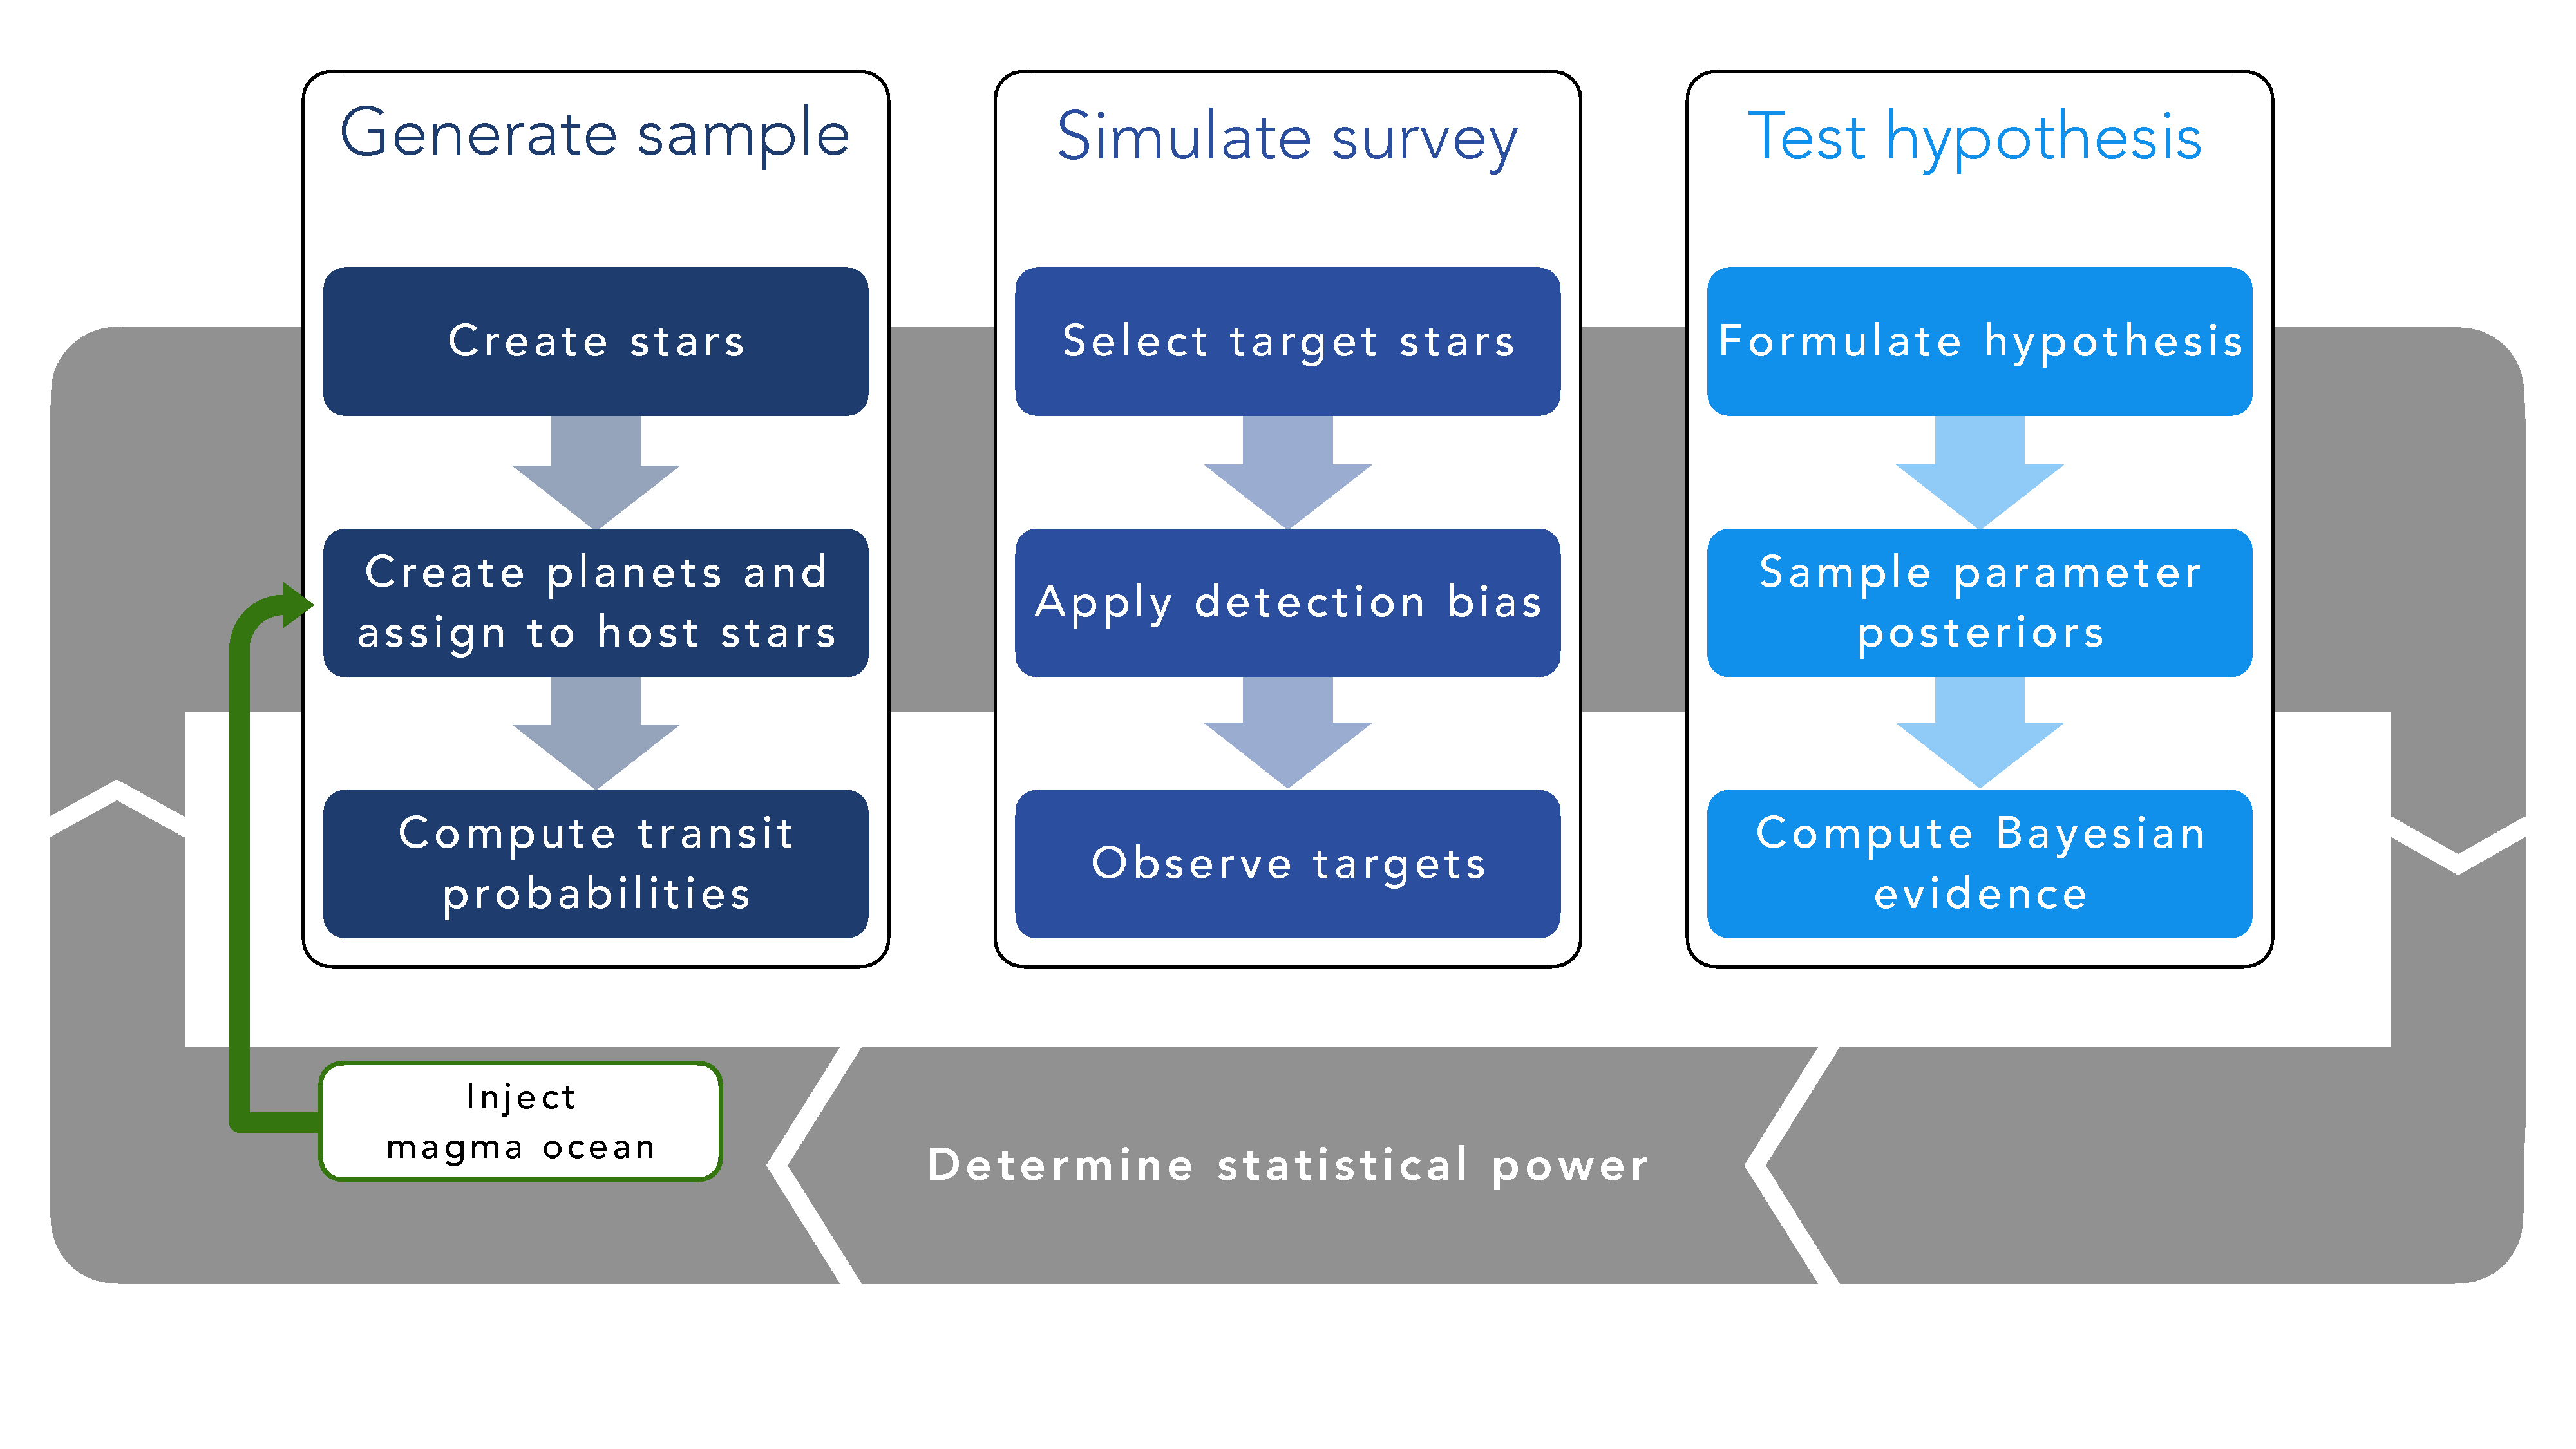
\includegraphics[width=\hsize]{figures/flowchart.pdf}
        \caption{Workflow of our hypothesis testing with Bioverse. In the first block, a stellar sample is generated based on XXX. The stars are then populated with planets from XXX, which may be assigned a magma ocean based on the model described in Sect.~\ref{sec:mo_model}. The planets' respective transit probabilities are computed. The second block simulates the exoplanet survey whereby selection effects and detection biases are introduced. Finally, the third block deals with testing a hypothesis based on the data from the simulated survey. By iterating through these steps, we compute the statistical power of testing the hypothesis given the assumed survey design.}
        \label{fig:flowchart}
    \end{centering}
\end{figure*}


\subsection{Synthetic star sample}
The first step in our analysis is to generate a synthetic sample of stars and planets.
First, we created a stellar population based on the observed population in the solar neighborhood, to which we then assign planetary systems based on occurrence rates derived from the \kepler\ mission.

\subsubsection{Stellar sample from Gaia DR3}
Different sample sizes are realized by varying the maximum distance of stars to the solar system $d_\mathrm{max}$.
\todo[inline]{KEVIN: describe stellar population}

\subsubsection{Stellar luminosity tracks}
    Planetary systems are hosted by stars of a wide range of ages, and stellar luminosities evolve with time.
    Since the emergence of a runaway greenhouse phase on a planet is highly dependent on the level of radiation it receives, and thus on the luminosity of the host star, we assigned age-dependent luminosities to our synthetic stars.
    Stellar ages are notoriously poor-constrained (CITE); we thus drew random ages from a uniform distribution from \SI{0}{\giga\year} to \SI{10}{\giga\year}.
    We then assigned each star a luminosity from the mass-dependent evolutionary models in \citet{Baraffe1998}.
    Figure~\ref{fig:luminosity_tracks} shows the corresponding luminosity evolution as a function of stellar mass and age.
\begin{figure}[ht!]
    \script{plot_luminosity_tracks.py}
    \begin{centering}
        \includegraphics[width=\linewidth]{figures/luminosity_tracks.pdf}
        \caption{
            Bolometric luminosity tracks of stars with different masses, computed from stellar evolution models in \citet{Baraffe1998}.
            Low-mass stars, which make up the majority of stars in the solar neighborhood, undergo an extended early phase of several magnitudes higher luminosity before entering a lifetime of relative faintness.
        }
        \label{fig:luminosity_tracks}
    \end{centering}
\end{figure}

\subsection{Synthetic planet sample}\label{sec:syn_planets}
Next, we assigned planetary systems to the synthetic stellar sample.
The orbital parameters and bulk properties of these simulated planets are informed by statistics from the \kepler\ mission.

\subsubsection{Planet occurrence rates in orbital period and radius}
We adopted the planetary occurrence rates recently derived in \citep{Bergsten2022}.
Following \citep{Youdin2011a}, their inferred occurrence rate density can be expressed in the form
\begin{equation}
    \frac{\mathrm{d}^2n}{\mathrm{d}R \, \partial P} = F_0 C_n g(R, P),
\end{equation}
where $F_0$ ...
\todo[inline]{GALEN: Describe underlying planet occurrence rates of synthetic population, its Mstar dependency, any caveats or assumptions.}


\subsubsection{Eccentricities, orbital inclinations, and planet masses}
Eccentric orbits alter the probability of a planet to transit \citep[e.g.,][]{Barnes2007a}.
The distribution of eccentricities $e$ of exoplanets has been found to resemble a Beta function \citep{Kipping2013b}, which we chose to draw synthetic eccentricities from.
Following~\citet{Kipping2013b}, we used a Beta distribution with parameters $a=0.867$ and $b=3.03$, and truncated the distribution at $e = 0.8$.

Another parameter with an even higher impact on transit probabilities is the orbital inclination toward the observer $i$.
Assuming isotropic alignments of orbits, we assigned each planet an inclination drawn from a distribution uniform in $\cos(i)$.

To assign masses to our planets, we use the semi-empirical mass-radius relationship derived in \citet{Zeng2016}.
The default relation our planets follow is one assuming a pure $\mathrm{MgSiO_3}$ composition.
\todo[inline]{JUSTIFY this choice (TIM?)}
This represents the baseline bulk density before any magma ocean-related effects are applied.


\subsubsection{Transit probability}
\begin{note}
    Not all planets are transiting from our point of view.
    We model the occurrence of transits by assuming random, isotropic orientations of planetary orbits and calculating the transit impact parameter $b = \cos(i)/R_\star$ for each planet.
    Only planets with $|b| < 1$ are potentially observable in transit and further considered.
    For these cases we calculate the transit depth
    \begin{equation}\label{eq:transitdepth}
        \delta = \left( \frac{R_\mathrm{P}}{R_\star} \right)^2
    \end{equation}\todo[inline]{check if transit depth or duration are actually used further down}
    and transit duration
    \begin{equation}\label{eq:transitduration}
        t_{\mathrm{T}} = \frac{R_\star P}{\pi a} \sqrt{1 - b^2},
    \end{equation}
    which are relevant for the detection probability of the respective planet~(see Sect.~\ref{sec:sensitivity}).
    Excluding all non-transiting planets diminishes the sample to \SI{\percentageTransiting}{\percent} of its original size.
\end{note}




\subsubsection{Synthetic planet populations with and without magma oceans}
\begin{note}
    Central to our procedure is to explore the detectability of population-level trends with future exoplanet surveys, and here the trend in question is the proposed radius discontinuity.
    To enable a quantitative assessment of this detectability, we injected the signal into the simulated planet sample before observing it with simulated surveys.
    While we search for the magma ocean pattern in demographic quantities such as average planet radii, the injected changes happen on the planetary level: We changed each planet's radius based on its individual set of properties and the associated predictions from steam atmosphere and water incorporation models.
    Relevant properties are a planet's mass $M$, its instellation $S$, and its bulk water inventory expressed as a water mass fraction $x_{H_2O}$.
    We consider three different cases:
    \begin{itemize}
   \item[A.] No radius change.
    This case serves as our null hypothesis, where planetary radii are not affected by the amount of irradiation the planets receive.
    It also applies outside the runaway greenhouse limit, where we assume a solid planetary surface and no steam atmosphere.
        A planet that lies \textit{within} the runaway greenhouse limit but that is already completely desiccated will have the same radius. \todo{Mention if this case is considered in the model or not (as of now, no).}
   \item[B.] Radius inflation due to a steam atmosphere.
    We assigned planets within the runaway greenhouse limit steam atmospheres, which increase atmospheric scale heights significantly.
   \item[C.] As B, but including radius decrease of inflated planets due to water in the melt.
    Due to greenhouse forcing, planetary surfaces below steam atmospheres are thought to be molten.
    Part of the water will then partition into the melt, removing it from the steam atmosphere, which in turn decreases the radius inflation.
    This effect is generally small compared to the radius inflation from a steam atmosphere but resulting radius changes typically reach measurable values.
    \end{itemize}
\end{note}


In case~A, a planet simply retains the radius it was assigned based on exoplanet occurrence rates (see Sect.~\ref{sec:syn_planets}).
There is no additional dependency on orbital distance or instellation.

Case~B assumes an inflated radius due to a steam atmosphere for all planets receiving a dayside-averaged instellation exceeding a threshold of $S_\mathrm{thresh} = \SI{280}{\watt\per\meter\squared}$.
This value was found to be a limit for the flux a planet can emit in a runaway greenhouse situation~\citep{Goldblatt2013,Leconte2013}.
To quantify the radius change, we applied the mass-radius relationships derived by \citet{Turbet2020} using a 1D~inverse radiative-convective model~\citep{Turbet2019}.
For the rocky interiors, their calculations rely on the same mass-radius relations from ~\citep{Zeng2016} that we applied for case~A-planets.
For each planet above the instellation threshold, we assigned the predicted radius for the given water mass fraction and planet mass.
We note that an additional radius change due to potentially molten interiors~\citep{Bower2019} is not taken into account here.

Case~C contains case~B, but also includes a radius decrease due to water partitioning in the melt.
The magnitude of this effect is again dependent on the planet mass and on the water mass fraction.
We follow \citet{Dorn2021} and use their computed radius deviations between a wet magma ocean and a solid mantle for a tropopause pressure~$P_\mathrm{iso}=\SI{0.1}{\bar}$.
We then add the (in almost all cases negative) radius deviations to the planet radii computed for case~B.

\begin{figure}
    \begin{centering}
        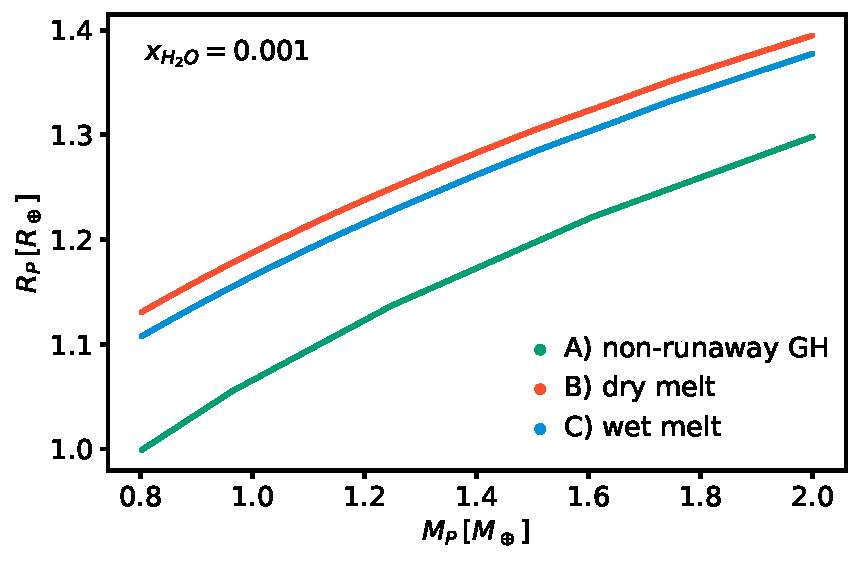
\includegraphics[width=\hsize]{figures/radiuscomparison.pdf}
        \caption{Mass-radius relationships for a water mass fraction $x_{H_2O}= \wrr$ and different planet states: A) fully solid planets without magma oceans. B) planets with steam atmospheres. C) As B), but including the effect of water incorporation in the melt.}
        \label{fig:radiuscomparison}
    \end{centering}
\end{figure}

Figure~\ref{fig:radiuscomparison} shows the different mass-radius relations of the three cases for a fiducial water mass fraction of $x_{H_2O}= \wrr$.
In general, steam atmospheres (case~B) cause a significant radius increase, which is slightly reduced when water incorporation in the melt is allowed (case~C).
Our nominal simulation setup is such that all planets receiving an instellation $S < S_\mathrm{thresh}$ follow relation~A, and all planets with $S > S_\mathrm{thresh}$ follow relation~C.
This introduces a sharp discontinuity of average planet radii and bulk densities as a function of stellar irradiation.
In the following, we test if and under what conditions this trend is large enough to be detected with high significance.



\subsection{Testing the magma ocean hypothesis with current and planned exoplanet missions}
\todo{Introduce survey simulation(s). PLATO, Cheops, Ariel, LIFE (reach out to team; Hendrik Linz produced a LIFE Technology Overview document)?, Nautilus\\ What are threshold missions that are able to detect this signal? =>X meter working for Y years, or X' meter working for Y' years => conclusion could be that there is interesting science to do with intermediate size telescope.}
In previous steps, we generated a population of synthetic planets that orbit synthetic stars, and we have injected the statistical trend expected from the presence of magma oceans on a fraction of the planets.
Only a subset of these planets would be detectable by a transit survey, and their properties can be probed only with a finite precision.
To test the detectability of a runaway greenhouse transition, we simulated several transit surveys with different designs and strategies and explored their capability to recover the magma ocean trend and constrain its parameters.
We assessed this capability based on two determinants: the likelihood that the mission is able to detect the injected trend, and the precision with which it can constrain the parameters of that trend.

%We consider a number of key parameters of transit surveys: The telescope's mirror diameter (or effective diameter for a telescope array) $D$, the total time budget of the survey for observations $t_\mathrm{total}$, the maximum number of observed transits for each target $N_\mathrm{obs, max}$, the slew time between observations $t_\mathrm{slew}$, ... \todo[]{double-check which survey params are needed}
We identify the following drivers of the diagnostic power for detecting the runaway greenhouse transition with a given transit survey:
\begin{itemize}
    \item Prevalent water inventory: The magnitude of radius change at the runaway greenhouse threshold is highly sensitive on water mass fraction. As a result, the statistical abundance of water in terrestrial planets impacts the strength of the demographic pattern.
    \item Sample size: Since we are looking for a population-level trend, the statistical significance will increase with a larger sample size.
    \item Radius measurement precision: The more precise individual planet radii can be determined, the less smeared out the pattern will be. Good \textit{accuracy} is less important, as long as it does not have a systematic error scaling with stellar irradiance.
    \item Availability and precision of mass measurements: For simple geometric reasons ($\rho \propto R^{-3}$), the expected trend is stronger when measured in bulk density than it is in planet radius space. If transiting planets can be followed up to obtain mass measurements, the statistical significance increases.
\end{itemize}
Besides these main factors, uncertainties in the measured instellations can influence the result, although they are typically small due to the very precise orbital period measurements available for transiting planets.
    This can be different for young host stars when their ages can not be well constrained; in particular the long pre-main sequence phase of M~dwarfs shows a large variation in bolometric luminosity~(see Fig.~\ref{fig:luminosity_tracks}).


\subsubsection{Survey simulations}
\begin{note}
The survey module of Bioverse converts the synthetic planet sample into a set of uncertainty-laden measurements of some parameters of a subset of that sample.
   This task includes selection of the targets, application of any detection biases, and conducting simulated measurements.
   All of the above are specific to the particular survey.

Current and near-future missions focusing on Earth-sized planets target several host star spectral types, and their exact sample selection is based on specific mission objectives.
    We thus chose a broad selection function centered on general detectability of transits with state-of-the-art technology.




\end{note}



\subsubsection{Sample selection}
\begin{note}
    \todo[inline]{use criterion of Zahnle \& Caitling 2017 instead? $0.8 S^{0.25} < R$}
    The runaway greenhouse effect becomes obsolete where no atmosphere can be maintained due to proximity to the host star and resulting atmospheric erosion.
    We thus excluded planets with extremely high instellation that does not allow long-term preservation of an atmosphere and clear our sample from all planets with an instellation $S > \SI{2000}{\watt\per\square\meter}$.
    We further consider only rocky planets with masses below \SI{2}{\Mearth}. % (Turbet+2020 covers only 0.1 to 2 Mearth)
\end{note}










\subsubsection{Definition of the magma ocean hypothesis and null hypothesis}
\todo{Define the null and alternative hypotheses}
\begin{note}
    As a null hypothesis, we consider the case where the planetary radius distribution is independent of the instellation,
    \begin{equation}
        h_{\mathrm{null}}(\theta, S) = \theta,
    \end{equation}
    where $\theta$ is the set of parameters defining the radius distribution.
    We further define an alternative hypothesis that describes radius changes due to steam atmospheres and water in the melt.
    As motivated above, this hypothesis takes the form of a step function in instellation $S$, where the step occurs at the outer edge of the runaway greenhouse region.
    Our main observable shall be the average planet radius in the planet population inside and outside this threshold.
    The magma ocean hypothesis is then defined as
\begin{equation}
    h_{\mathrm{MO}}(\theta, S) =
%        \begin{cases}
%        1 & \text{if } x \in \mathbb{Q}\\
%        0 & \text{if } x \in \mathbb{R}\setminus\mathbb{Q}
%    \end{cases}
        \begin{cases}
        h_{\mathrm{null}} & \text{for } S \leq S_\mathrm{thresh}\\
        <R_\mathrm{P}> (f_\mathrm{steam}, f_\mathrm{water}) & \text{for } S > S_\mathrm{thresh}.
    \end{cases}
\end{equation}
    Here, $f_\mathrm{steam}$ and $f_\mathrm{water}$ are predictions from the steam atmosphere and water incorporation models, respectively.
    They are assumed to act additively on the planet radii and thus on their average $<R_\mathrm{P}>$.

%        \begin{cases}
%        \end{cases}

\begin{figure}
    \begin{centering}
        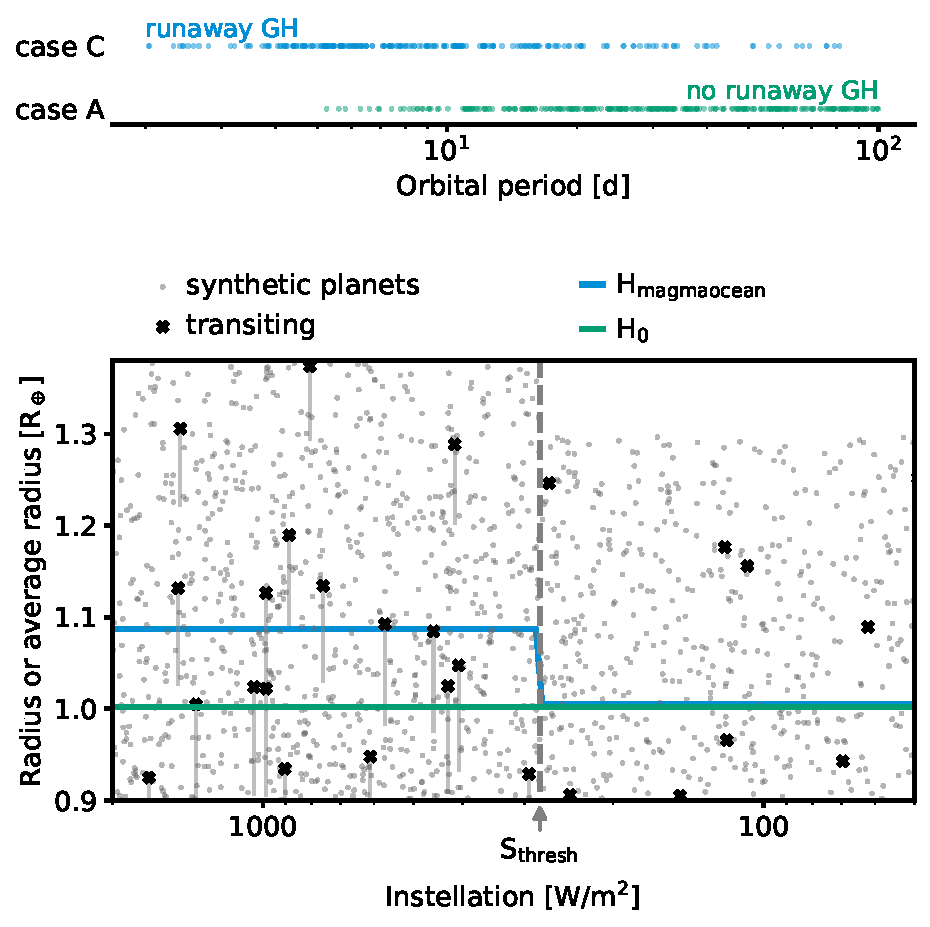
\includegraphics[width=\hsize]{figures/HnullHmo.pdf}
        \caption{Planets above and below the runaway greenhouse threshold.
        \textit{Top}: Planet state as a function of orbital period. Planets with and without a runaway greenhouse climate mix and are not distinguishable in period space.
        \textit{Bottom}: Radii of synthetic planets with injected radius deviation as a function of instellation. Only the planets marked as transiting are observable. Above the runaway greenhouse threshold $S_\mathrm{thresh} =\SI{280}{\watt\per\meter\squared} $, radii are inflated by the amount indicated with gray lines. The sharp boundary at $S_\mathrm{thresh}$ causes a discontinuity in the average planet radius (blue). This magma ocean hypothesis can be tested agains the null hypothesis $H_0$ (green), where average radii are independent of instellation.}
        \label{fig:HnullHmo}
    \end{centering}
\end{figure}
    Figure~\ref{fig:HnullHmo} shows the null and alternative hypotheses as a function of instellation.
    The value for the average radius \textit{outside} the runaway greenhouse regime was computed from our nominal observed sample, whereas the radius change in the magma ocean case compared to the null hypothesis is a prediction from the magma ocean model, evaluated on the same sample.

\end{note}

...

For the likelihood function, we assumed that the planet radii $R_{\mathrm{P}, i}$ are measured with a normally distributed uncertainty $\sigma_{R_\mathrm{P}, i}$ and adopted a normal distribution
\begin{equation}
    \mathcal{L}(R_\mathrm{P} \mid \boldsymbol{\theta})=\prod_{i}^{N} \frac{1}{\sqrt{2 \pi \sigma_{R_\mathrm{P}, i}^{2}}} \exp \left(-\frac{\left(R_{\mathrm{P}, i}-h\left(\boldsymbol{\theta}, a_{\mathrm{eff}, i}\right)\right)^{2}}{2 \sigma_{R_\mathrm{P}, i}^{2}}\right).
\end{equation}
Here, $h\left(\boldsymbol{\theta}, a_{\mathrm{eff}, i}\right)$ corresponds to the functional form of the magma ocean hypothesis\todo{link to eqn defining the hypothesis} .
We tested this hypothesis against the null hypothesis $h_\mathrm{null} (\theta, R_\mathrm{P}) = \theta$, which states that there is no relationship between the measured planet radii and (scaled) semi-major axes.

\subsection{Signature and testability of the magma ocean hypothesis with the PLATO transit survey}
PLATO (PLAnetary Transits and Oscillation of stars) is an ESA mission designed to characterize terrestrial planets in the habitable zones of Sun-like stars, a goal to be achieved via long-term high-precision photometric monitoring of a sample of bright stars~\citep{Rauer2016}.
The PLATO team has released an estimate on the number of exoplanets that will be characterized in the course of the main survey mission (Matuszewski, priv. comm.).
In the FGK sample of the mission, a minimum of 500 Earth-sized (\SIrange{0.8}{1.25}{\rEarth}) planets are expected to be detected.
We base our assessment of PLATO's diagnostic power to test the magma ocean hypothesis on these estimates.

\begin{figure}[ht!]
%    \script{figurescript.py}
    \begin{centering}
        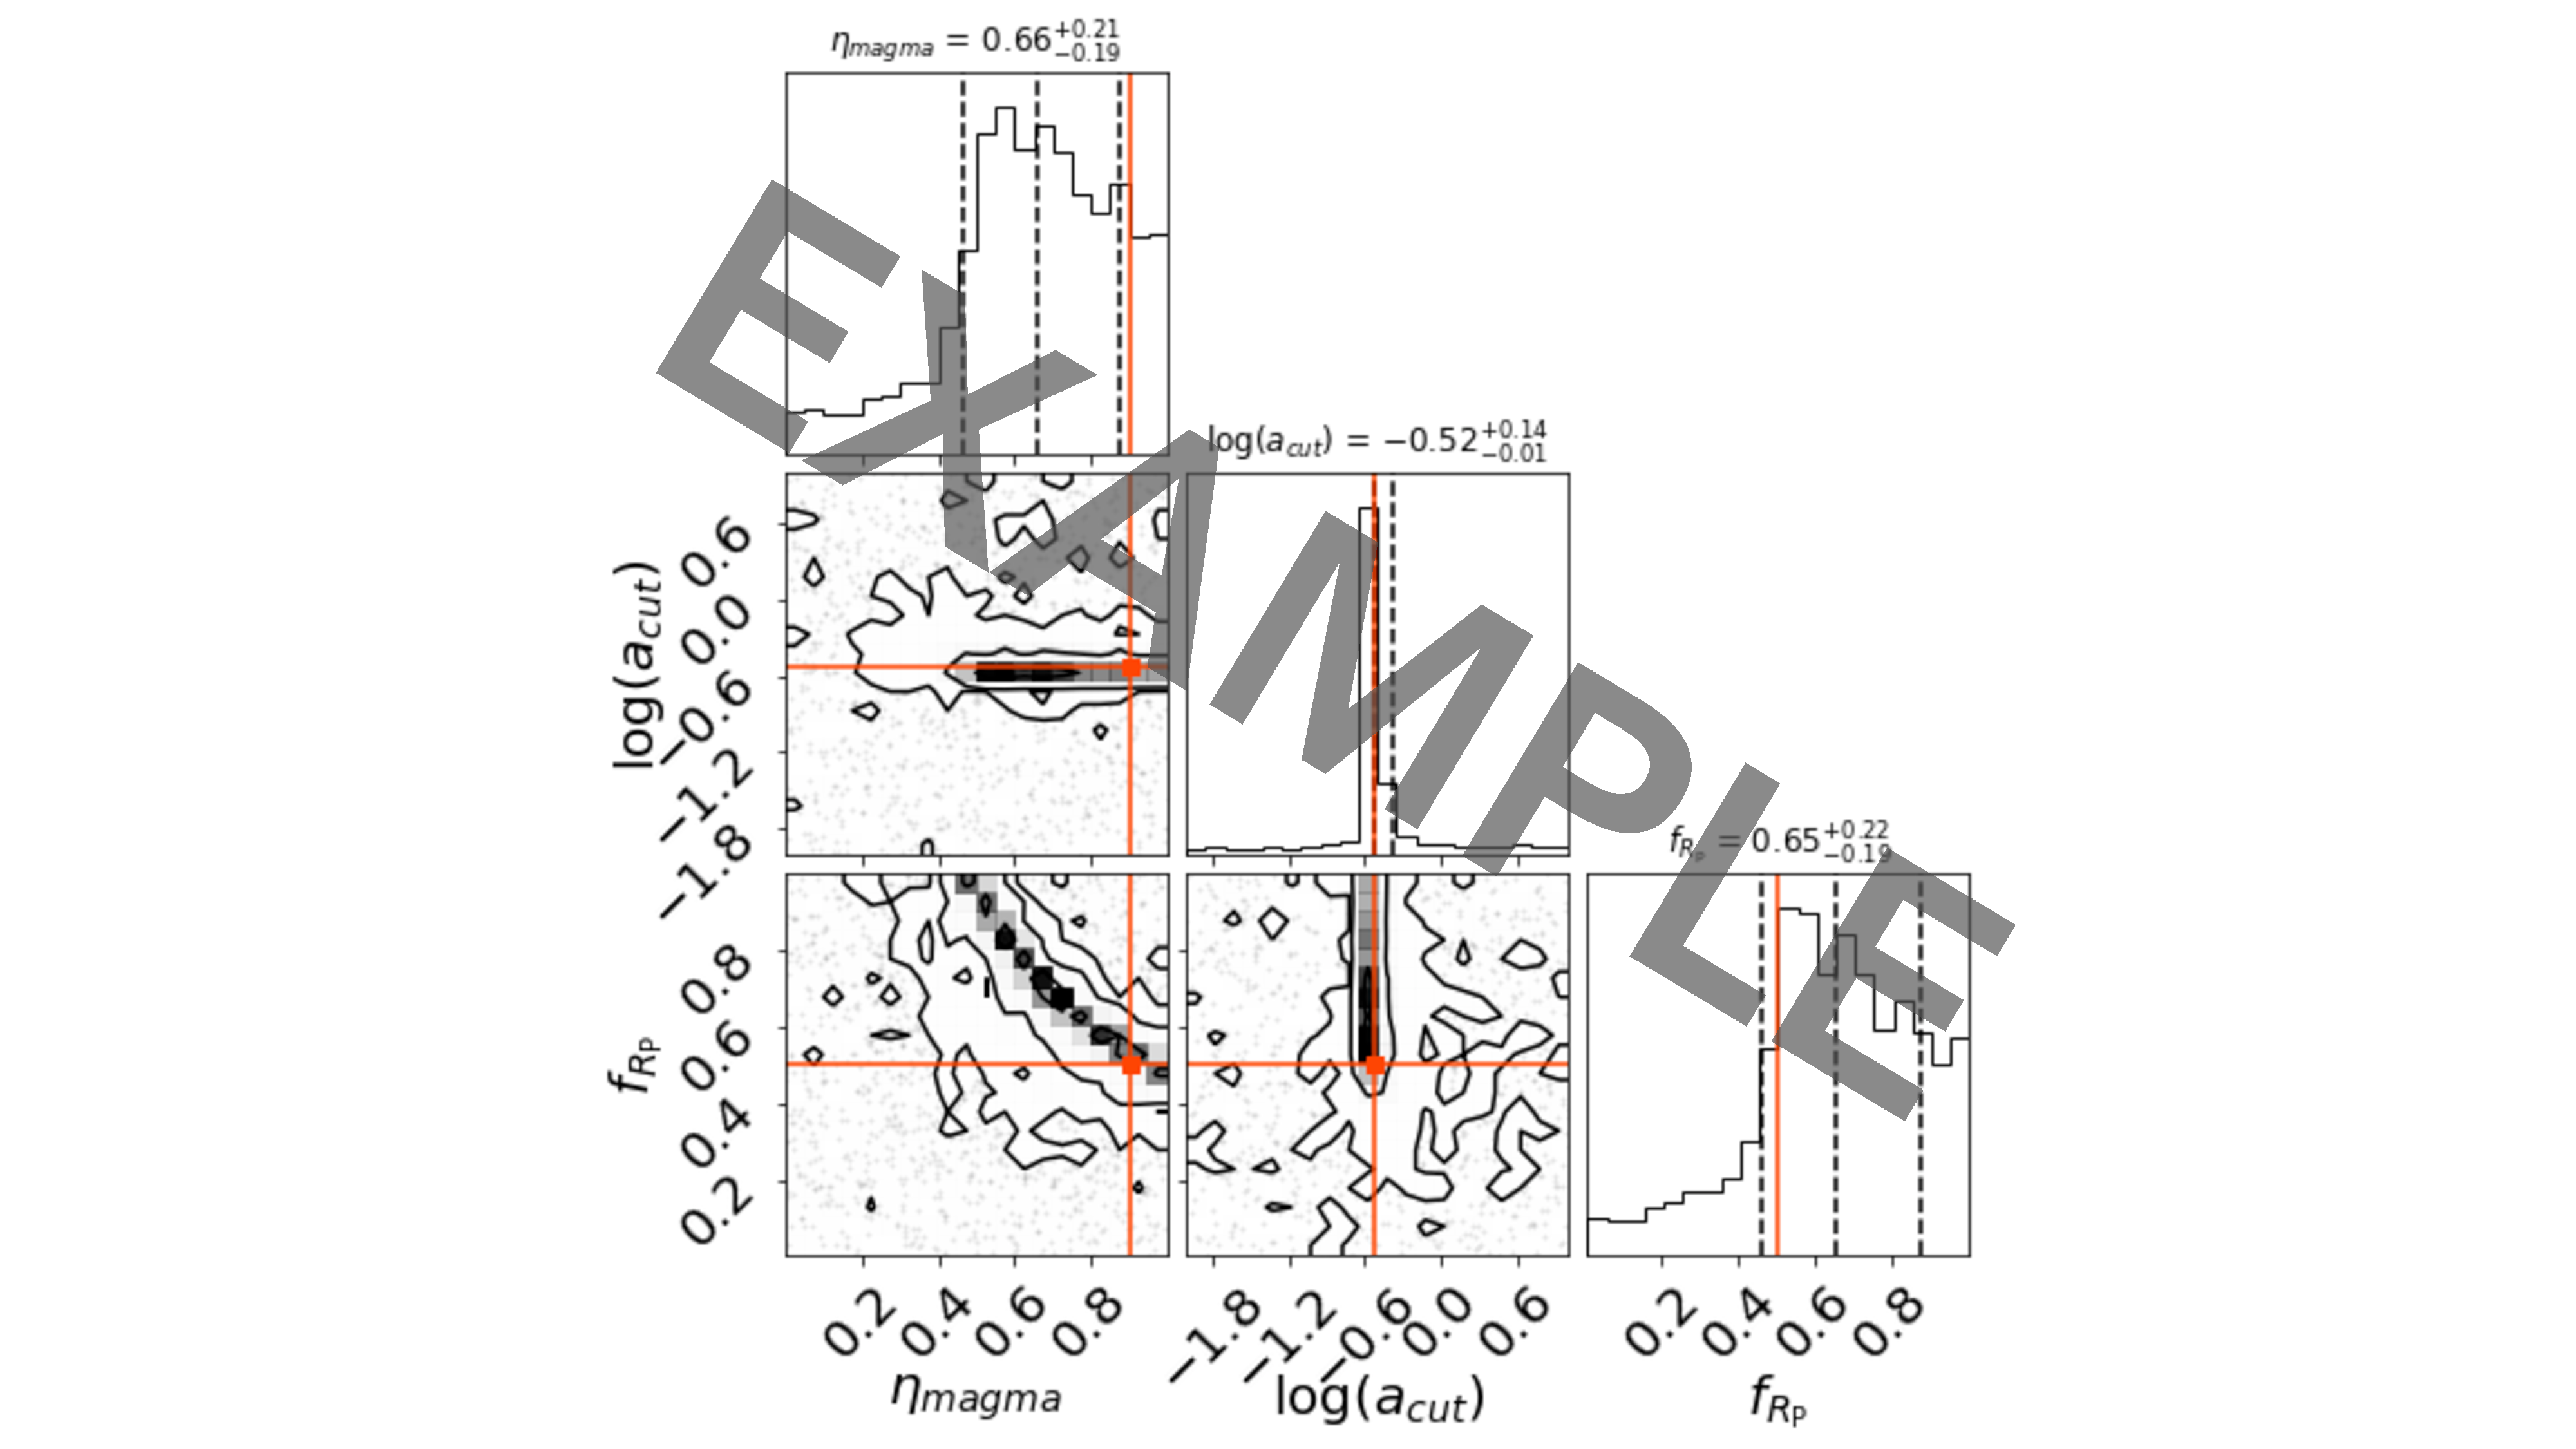
\includegraphics[width=\linewidth]{figures/example_cornerplot.pdf}
        \caption{
        Retrieved posterior distribution of magma ocean model. The density maps in each panel show relationships between and marginalized distributions of the model parameters as they would be retrieved with a targeted $<nominal telescope size>$ survey of $<survey duration>$ duration. True values of the injected magma ocean parameters are shown in orange. ...
        }
        \label{fig:cornerplot}
    \end{centering}
\end{figure}



\begin{note}
   The fidelity of a future detection or falsification of a magma ocean signature will depend on the significance with which the null hypothesis can be excluded.
   As a consequence, instrumentation and survey strategy aiming at testing the hypothesis should aim at maximizing the probability of a true positive detection given the existence of the effect.
   This is called the statistical power of the test.
   Before turning to mission design trades that influence the statistical power in Sect.~\ref{sec:mission-design-trades}, we explore its behavior as a function of various free parameters of the magma ocean model.
    ...
\begin{figure*}[ht!]
%    \script{figurescript.py}
    \begin{centering}
        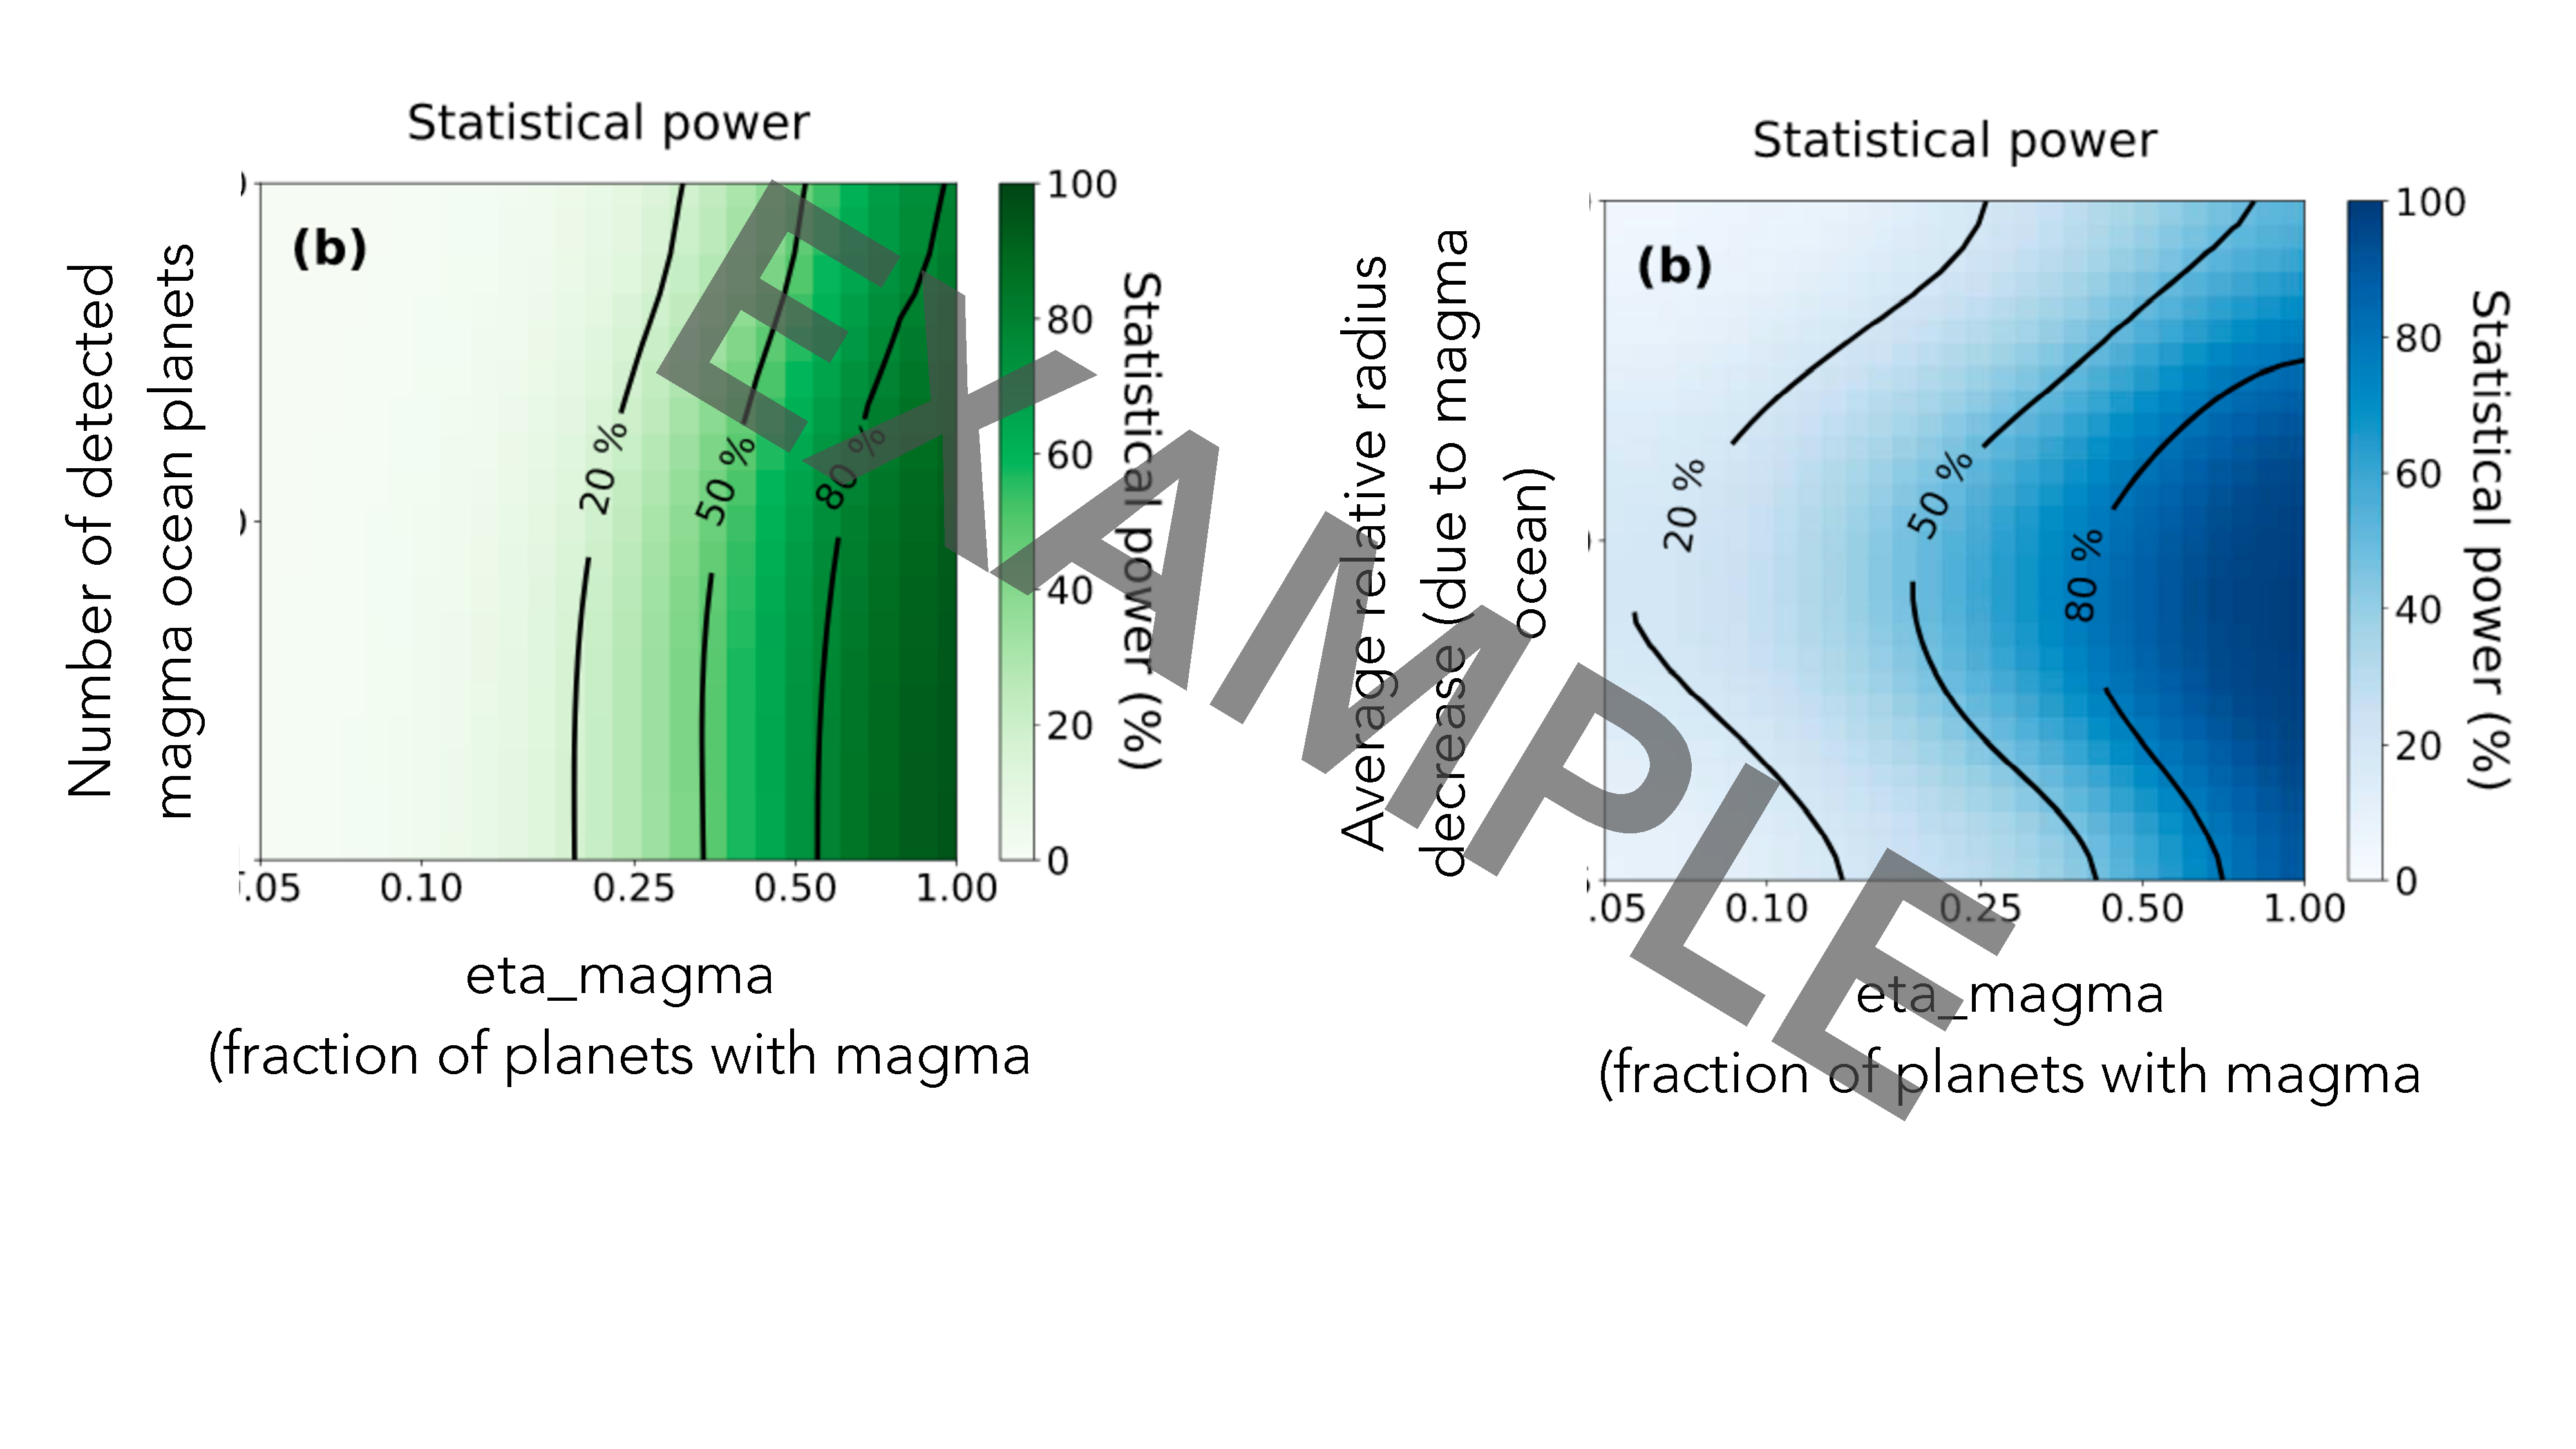
\includegraphics[width=\linewidth]{figures/example_statistical_power.pdf}
        \caption{
        Statistical power of a magma ocean hypothesis test as a function of model parameters.
        }
        \label{fig:statistical_power}
    \end{centering}
\end{figure*}

\end{note}

\subsection{Statistical power of different mission designs}\label{sec:statpower_missions}
\todo[inline]{show detectability of the magma ocean signature for different mission designs}

\begin{figure}[ht!]
%    \script{figurescript.py}
    \begin{centering}

        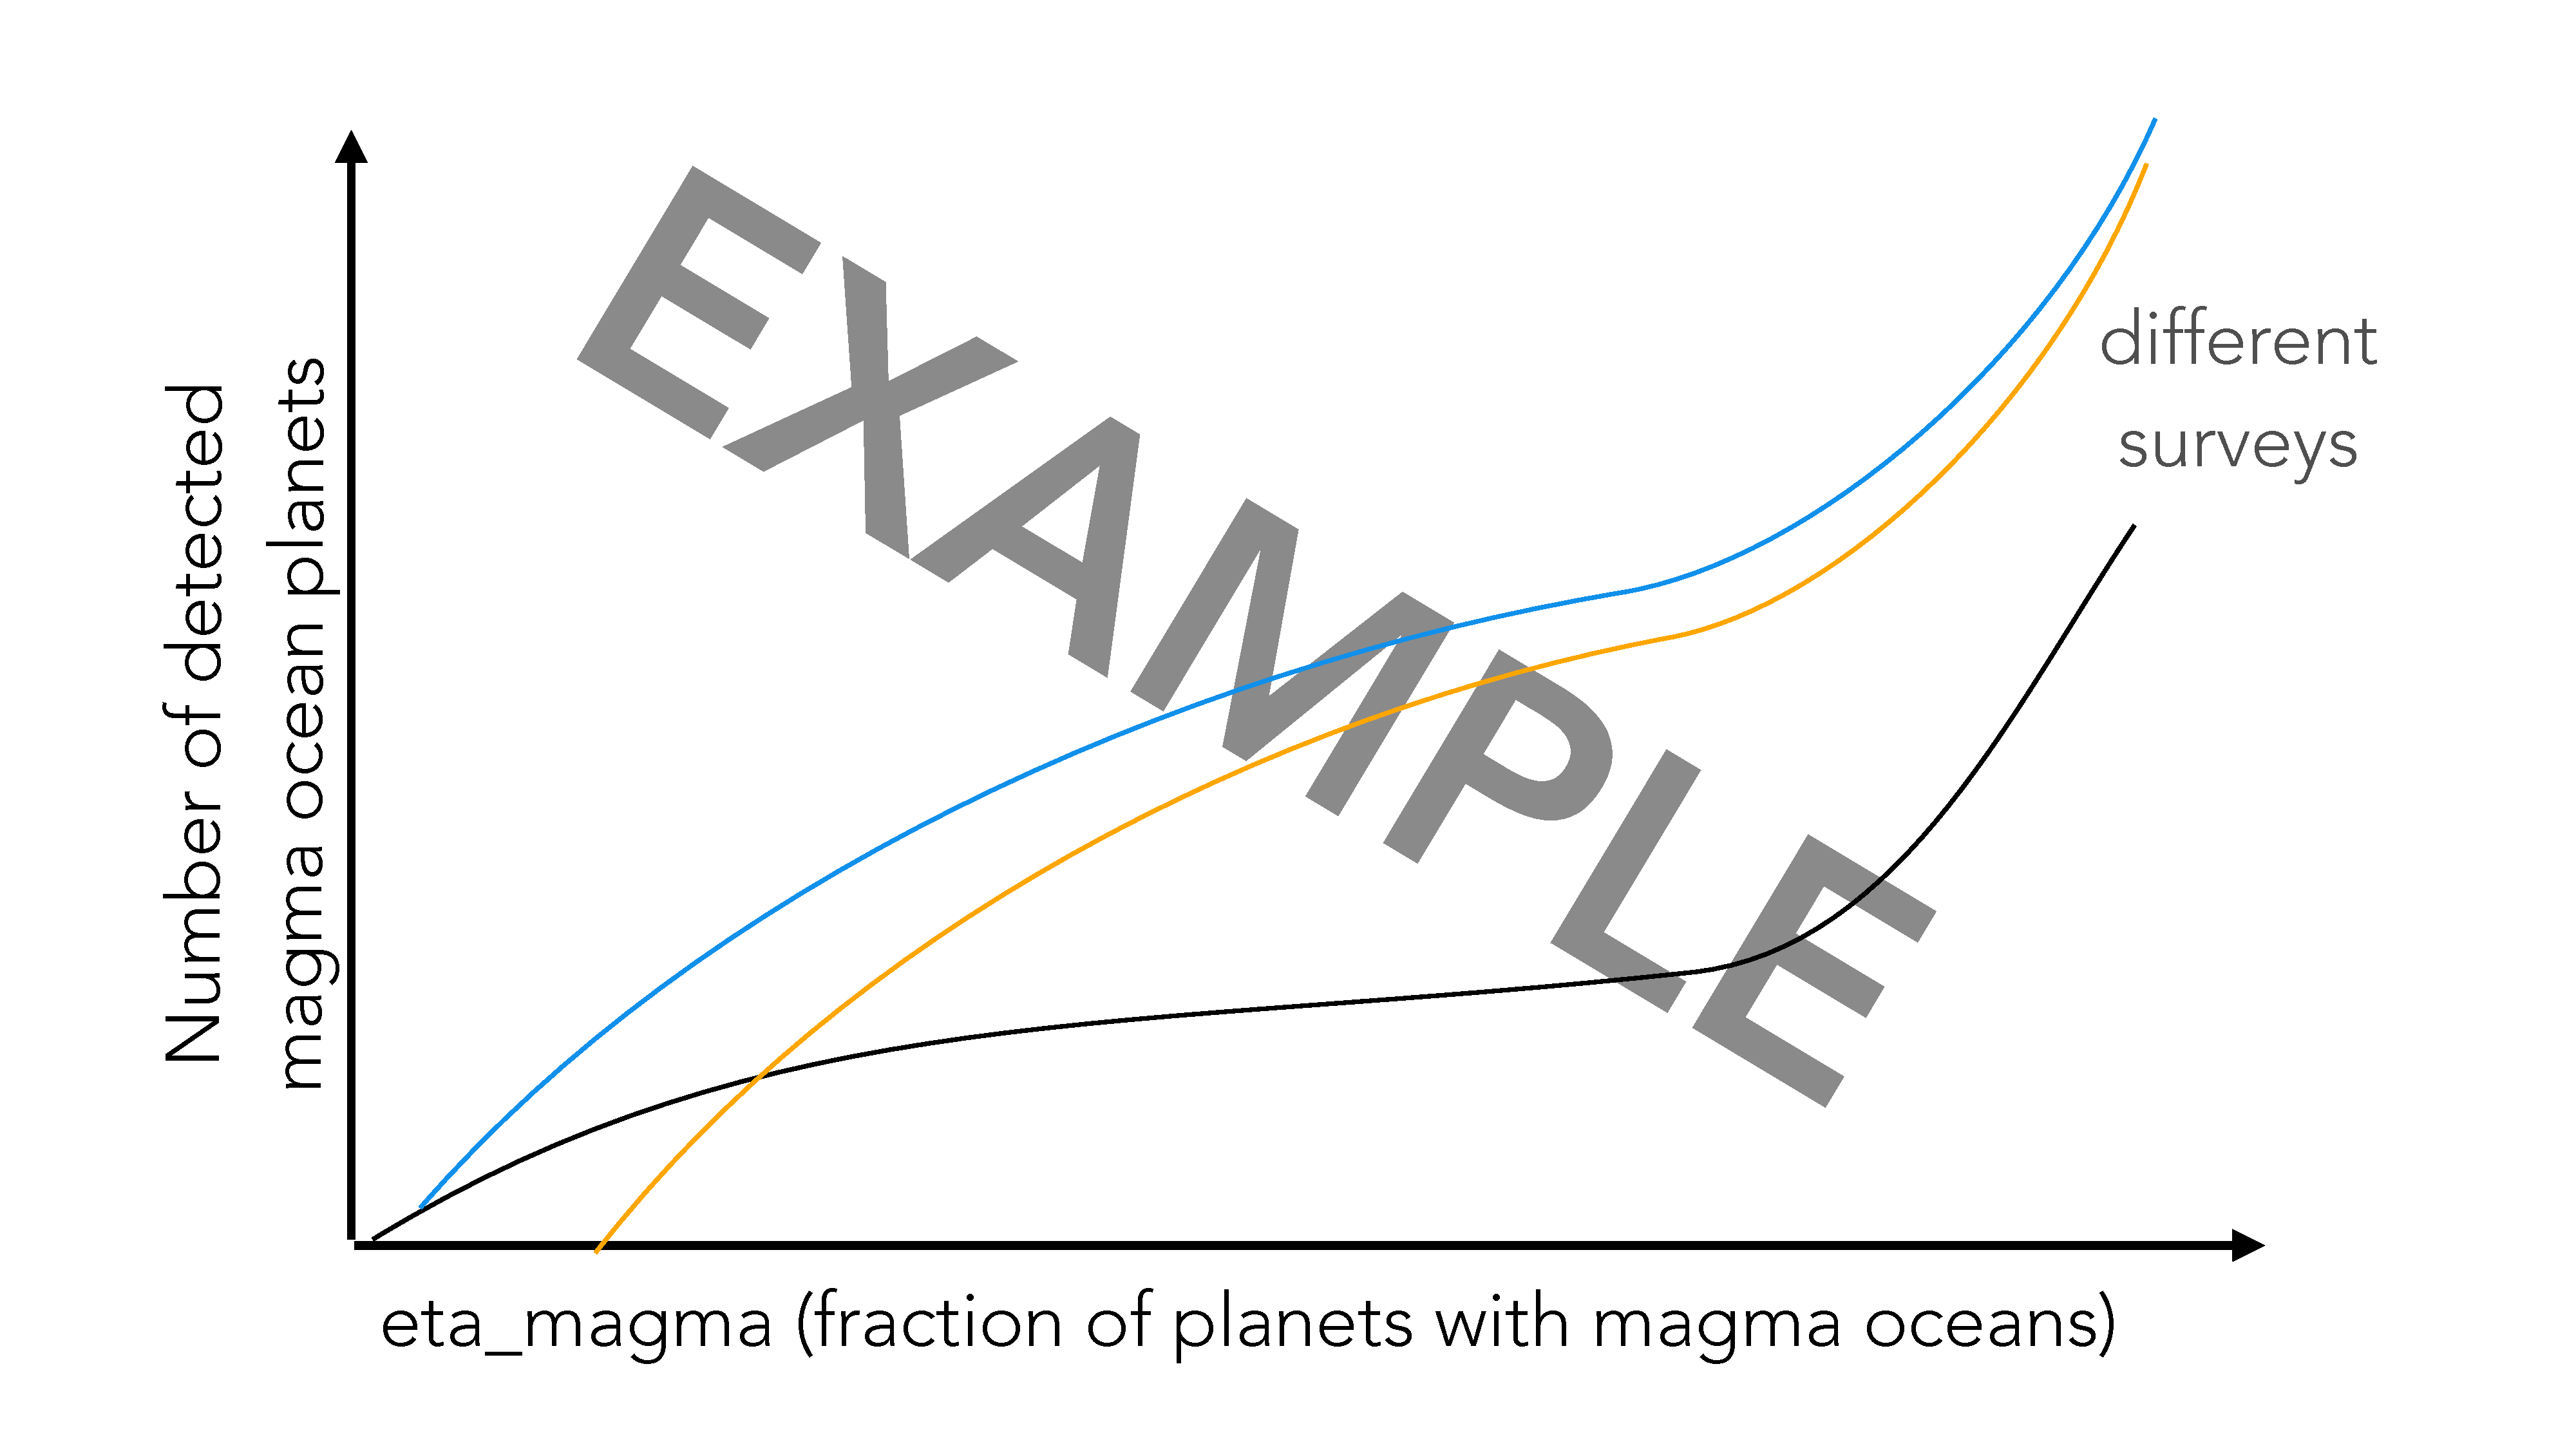
\includegraphics[width=\linewidth]{figures/example_Ndetected_surveys.pdf}
        \caption{
        Detections of magma ocean-bearing planets as a function of magma ocean occurrence for different survey designs.
        }
        \label{fig:example_Ndetected_surveys}
    \end{centering}
\end{figure}

\section{Discussion}\label{sec:discussion}
\todo[inline]{\textbf{Potential discussion points: } what is the fraction of Kepler planets w/ runaway GH.}
\subsection{Expected imprint of runaway greenhouse phases on exoplanet demographics}

\subsection{Detectability of the magma ocean demographic feature}

\subsection{Diagnostic power of upcoming exoplanet missions}\todo[inline]{PLATO: needed sample size, precision}

\subsection{Mission design trades}\label{sec:mission-design-trades}

\subsection{Implications for planetary habitability}\label{sec:habitability}
\todo[inline]{Magma oceans influence the amount of water available at the surface and atmosphere, which is 1. commonly used as environmental marker to assess habitability, and 2. influences the planet's climate (greenhouse effect).}

\subsection{OPTIONAL...: Atmospheric signatures}
\todo[inline]{discuss potential atmospheric signatures of magma oceans. e.g.: H/O ratios of sub-Neptunes could be low (because H is in the melt) (Tim's talk)}

\subsection{False positive scenarios}
\todo{what other processes could be confused with a magma ocean signal?}
\begin{note}
Global magma oceans are not the only physical mechanism that may cause a decrease in transit radii for a subset of planets.
Other causes of shrinking planet sizes have been put forward, the most widely discussed ones being atmospheric loss due to either photoevaporation through high-energy radiation by the host star~\citep[e.g.,][]{Owen2013,Jin2014,Mordasini2020a} or due to residual heat from the planet's interior shortly after formation~\citep{Ginzburg2016b,Ginzburg2018,Gupta2019}.
    Both processes are being traded as potentially sculpting the observed radius bimodality of small, close-in exoplanets from the  mission~\citep{Fulton2017,VanEylen2018}.
    Like the magma ocean effect discussed here, these processes reduce the radii of some planets, leading to a decrease in average measured planet radii in a specific region of the planetary parameter space.
    This region is distinct from the one affected by global magma oceans, since... \todo{...elaborate why they cannot be confused}

    Another false positive contribution may come from potential unknown variations in the occurrence rate gradients in radius-instellation space.
    They can impact the statistical inference of the transitions, especially if these variations are similar to the expected pattern.
    Although an abrupt pattern at the expected runaway greenhouse transition seems unlikely, examples of steep occurrence rate density changes exist.
    An example is the "Neptune desert``, a triangular region of low planet occurrence density of close-in planets in period-radius space~\citep{Szabo2011,Mazeh2016,Dreizler2020b}.
    The shape of this region is such that smaller planets become less frequent the closer to the star they are, which to some degree resembles the pattern introduced by the instellation dependency of the magma ocean probability.
    However, the Neptune desert occurs at smaller orbital periods and its location depends on a planet's size~\citep{Szabo2011}, which is not expected for the runaway greenhouse transition.
    \todo{is there overlap/confusion with the radius/density trend in \citet{Luque2022b}?}
\end{note}

\todo[inline]{Maps to Sect. \ref{sec:statpower_missions}.}

\begin{note}
    \citet{Penny2019} mention that a significant increase in planet yield could be achieved if the telescope's slew speed was increased.
\end{note}

\begin{figure}[ht!]
%    \script{figurescript.py}
    \begin{centering}

        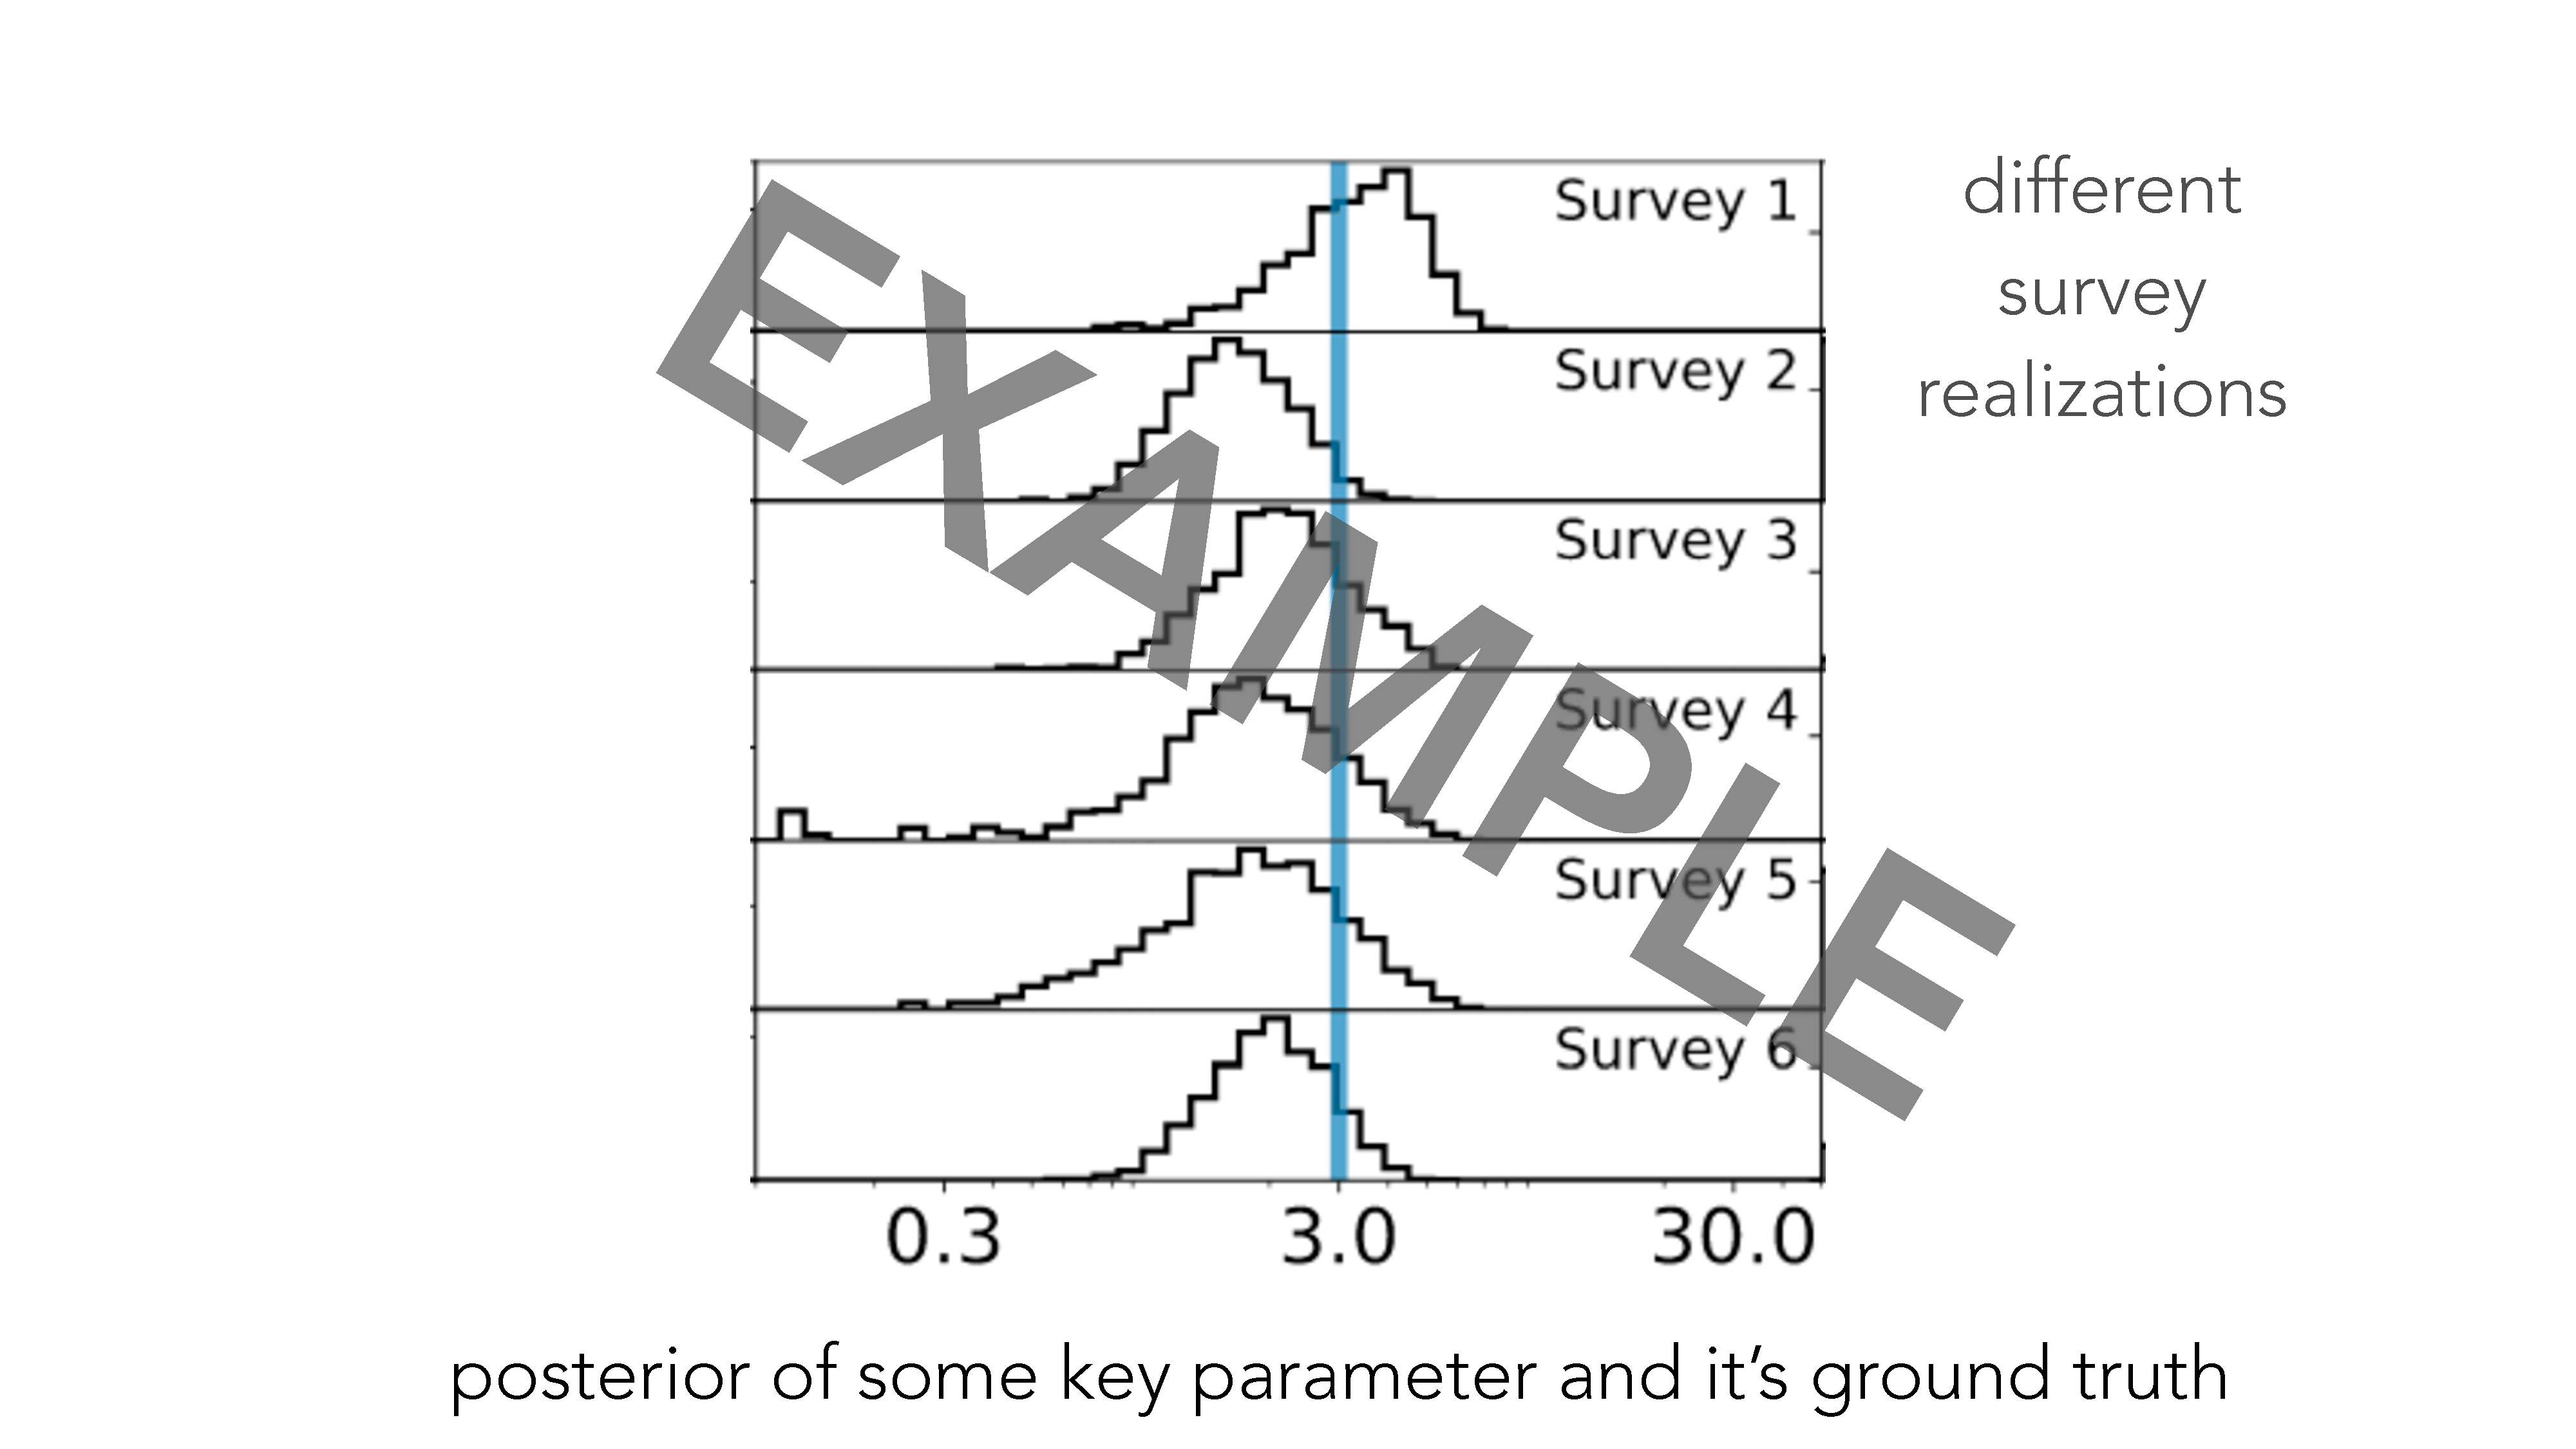
\includegraphics[width=\linewidth]{figures/example_posterior_surveys.pdf}
        \caption{
        Retrieved posterior distribution of the $<key parameter>$ for different survey realizations.
        The orange line corresponds to the true value of the injected signal.
        }
        \label{fig:posterior_surveys}
    \end{centering}
\end{figure}



\section{Conclusions}

\begin{note}
    \textit{Here or in the introduction:} For observations of rocky exoplanets, the currently best-probed regime is that of warm, close-in planets.
    These bodies experience climatic conditions that are similar to the environment of the inner Solar System bodies at early stages of their formation.
    Studies of the geophysical state and evolution of hot exoplanets can thus contribute to our understanding of the early formation stages of Earth and other habitable worlds.
\end{note}

The key findings of our work are as follows:
\begin{enumerate}
    \item Planetary radius changes due to the combined effect of steam atmospheres and water dissolved in the molten mantle of planets within the runaway greenhouse threshold is expected to cause a discontinuity in the radius distribution of small (DEFINITION) exoplanets.
    \item Since XXX\SI{}{\percent} of confirmed exoplanets in this size range are in the runaway greenhouse regime, we suggest that this imprint is detectable with transit measurements of a large enough sample and sufficient precision.
    \item Using Bioverse, we find that the planned PLATO transit survey will provide a sufficient sample to test the magma ocean hypothesis.
    \item The diagnostic power of transit missions in testing this hypothesis can be maximized by ...
    \item A detection of the feature will constrain the water inventory of rocky exoplanets, providing important context in the assessment of their habitability.
\end{enumerate}

%\begin{acknowledgments}
%The authors thank Yann Fabel, Paul Molliere, and Terry-Ann Suer for insightful discussions.
%We are grateful to Martin Turbet for providing the mass-radius relationship data for planets harboring steam atmospheres.
%\end{acknowledgements}

\begin{large}\textit{Author contributions:}\end{large}

\section*{Data Availability}
All data sets and software required to reproduce our results and this article are available through GitHub and Zenodo.
The code to reproduce the figures can be accessed via the icon links associated with the respective figure caption.


\software{
Bioverse~\citep{Bixel2021},
Astropy~\citep[][]{AstropyCollaboration2018},
NumPy~\citep[][]{Harris2020},
SciPy~\citep[][]{Virtanen2020},
corner.py~\citep{Foreman-Mackey2016b},
dynesty~\citep{Speagle2020}.
}


\bibliographystyle{aasjournal}
\bibliography{bib,PhD}
\end{document}